% Copyright (c) 2014,2016,2018 Casper Ti. Vector
% Public domain.

\chapter{单元测试与集成测试}
%\pkuthssffaq % 中文测试文字。
这一章主要进行正确性测试,分为单元测试和集成测试两个部分进行,分别在 \ref{sec:unit_test}小节和 \ref{sec:gen_test}小节进行介绍。
单元测试部分只测试我们实现的 exFAT 模块的正确性,测试的方式是模拟用户使用文件系统的操作,对实现的 exFAT 文件系统进行了
一系列的功能调用并检查正确性(功能调用和正确性检查都只会通过文件系统提供的接口进行)。
为了单元测试能进行得更充分,更好的模拟一般用户的使用,除了对文件系统的一些基本调用序列测试外,我们还设置了一项随机操作序列测试。
我们为这项测试实现了一个自动化随机测试单元,每次调用可以自动随机生成一组操作序列进行测试并检查正确性,\ref{sec:auto_test}小节详细介绍了这个测试单元。
集成测试则是将实现的 exFAT 作为操作系统的一部分,测试整个操作系统的正确性,这里我们用到了一些现有的集成测试模块。

\section{单元测试}\label{sec:unit_test}
这一节介绍基本单元测试。
我们使用内存模拟块设备,并使用一个已经被格式化的 exFAT 文件系统镜像进行初始化,
随后,针对文件系统提供的各种接口分别编写相应的测试样例,下面列出了所有的测试样例。

\begin{itemize}
    \item new\_exfat: 测试能否正确挂载 exFAT 文件系统。 
    \item create: 测试基本的创建功能,包括创建文件或目录、尝试创建同名文件、创建长名字文件。 
    \item create\_and\_list\_file: 测试列出文件功能,在该测试中,随着创建文件不断执行列出命令,检查能否完整列出所有文件。 
    \item unlink\_single\_file: 测试删除文件功能,包括删除普通文件、删除长名字文件、尝试使用 unlink 删除目录等。 
    \item unlink\_multiple\_files: 测试删除文件功能,在该测试中,首先创建一系列文件,随后随着删除文件不断执行列出命令,检查列出结果是否正确。 
    \item rmdir: 测试删除目录功能,与删除文件的测试类似,额外测试了尝试删除非空目录。 
    \item rename\_file: 测试重命名文件功能,包括重命名后的文件能否正常读写、重命名后的文件能否被正常列出、通过重命名进行不同目录之间的移动、重命名文件到存在的名字等。 
    \item rename\_dir: 测试重命名目录功能,包括重命名后子目录是否一致、重命名目录到存在的名字等。 
    \item write\_and\_read\_file\_direct: 测试直接读写文件,不使用页缓存,通过写入后再读出检查正确性。 
    \item write\_and\_read\_file: 测试读写文件,使用页缓存,通过写入后再读出检查正确性。 
    \item interleaved\_write: 测试交替写两个文件,模拟一些多文件工作场景。 
    \item bitmap\_modify\_bit: 针对 Bitmap 模块进行测试,测试修改其中的单个位。 
    \item bitmap\_modify\_chunk: 针对 Bitmap 模块进行测试,测试修改其中的连续若干位。 
    \item bitmap\_find: 针对 Bitmap 模块进行测试,测试寻找连续若干空闲位的功能。 
    \item resize\_single\_file: 测试针对单个文件的改变大小,包括均匀扩张和收缩、非均匀扩张和收缩、一次性分配过多空间、恰好分配所有剩余空间。 
    \item resize\_multiple\_files: 测试针对多个文件的改变大小,不同文件交替进行。 
    \item resize\_and\_write: 测试改变大小和写操作的兼容性,不断在调整文件大小后进行写。 
    \item random\_op\_sequence: 随机操作序列测试,详见\ref{sec:auto_test}小节。 
\end{itemize}

图\ref{fig:unit_test}展示了单元测试的结果,可以看到,我们实现的 exFAT 文件系统可以通过所有的测试。

\begin{figure}[h]
    \centering
    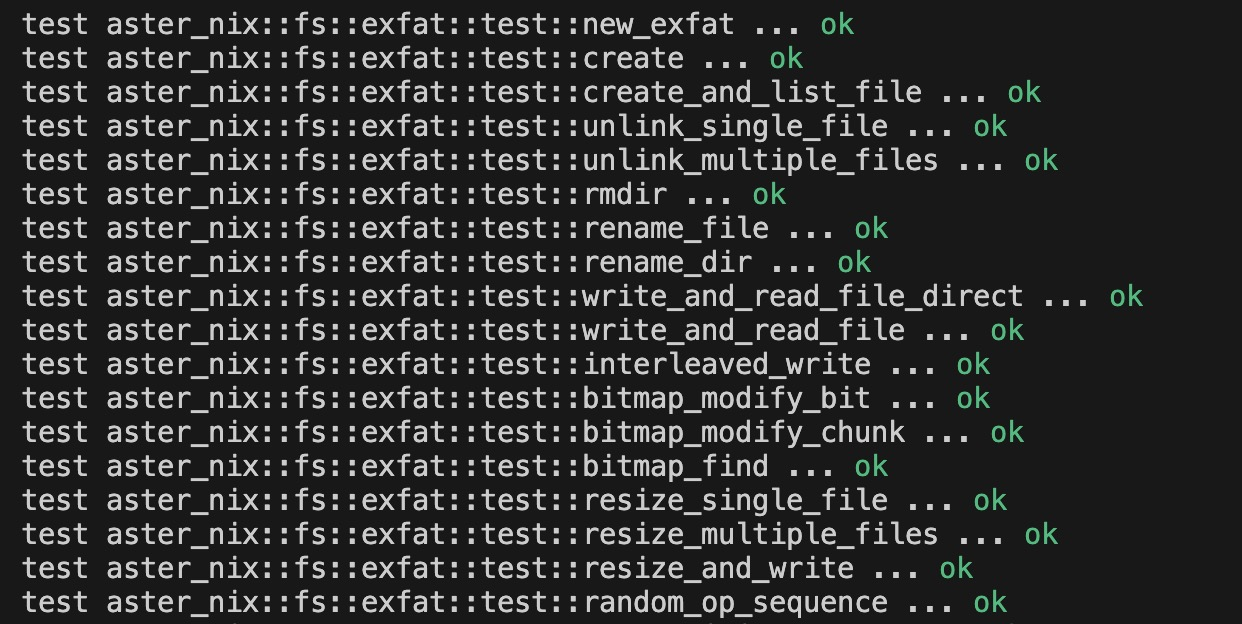
\includegraphics[width=1.0\textwidth]{chap5_unit_test.jpg}
    \caption{单元测试结果}
    \label{fig:unit_test}
\end{figure}

\section{自动化随机测试单元}\label{sec:auto_test}
这一节介绍为测试文件系统正确性设计的自动化随机测试单元。
通过这个测试单元,使用者只需指定期望执行的操作总数,测试单元即可自动生成一系列合法操作,执行并检查正确性。

为了检查正确性,这个测试单元在内存中维护一个文件系统的状态。
具体来说,我们在内存中维护了一颗目录树的结构,树上的每个节点都对应文件系统中的某个具体文件或目录。
针对目录,我们维护的状态包括当前目录名、所有子目录名以及作为目录树的内部节点必不可少的子节点的引用。
针对文件,我们维护的状态包括文件名和文件内容。
此外,为了方便的进行文件系统相关调用,我们在目录树上的每个节点里额外维护了对应的文件或目录在文件系统里的索引节点的引用。
于是当我们希望进行文件系统的调用时,可以直接通过节点上存储的索引节点引用进行。
进行测试时,测试单元根据自身维护的“文件系统”当前状态随机生成操作,向待测文件系统提交生成的操作,并利用自身维护的状态进行正确性检测。
从生成操作开始,到执行操作并检验结束,称为一次测试。

从上面的描述可以看出,测试单元最主要的两个功能分别是根据当前文件系统状态随机生成操作和检验待测文件系统执行操作的正确性。
下面分别介绍这两个功能如何实现。

\subsection{操作的生成}
为了确保测试更能反应用户实际使用的情况,我们希望随机测试单元生成的操作是合法的。
关于非法操作并没有过多测试的意义,在\ref{sec:unit_test}小节中介绍的单元测试已经针对非法操作进行过测试。
所以,在生成操作时,随机测试单元必须考虑到文件系统的当前状态。

操作由当前待操作的节点(具体的文件或目录,与当前文件系统状态有关)和对节点执行具体操作(如创建或删除文件、读写文件等)组成。
生成操作的流程大致是:先根据测试单元自身维护的当前文件系统状态选择希望执行操作的节点,而后针对前一步选择的节点生成待执行的操作。
下面是生成操作的伪代码。

\begin{algorithm}[H]
    \SetAlgoLined
    \KwData{描述文件系统当前状态的目录树 dir\_tree}
    \KwResult{待操作的节点 node,对节点执行的操作 operation}
    初始化 node 为目录树 dir\_tree 的根节点 \;
    \While{node 有孩子节点} {
        随机获取一个布尔值,得到真的概率可以视情况调整,这里使用了 50\%,表示是否希望继续深入目录树 \;
        \eIf{决定继续深入目录树}{
            赋值 node 为当前 node 的随机子节点 \;
        }{
            \textbf{break}\;
        }
    }
    至此我们随机从树上选取了节点 node \;
    针对刚刚随机获得的节点 node 随机生成一个合法操作 operation \;
    \textbf{return} (node, operation) \;
    \caption{随机生成文件系统的合法操作}
\end{algorithm}

\subsection{执行操作并检验正确性}
这部分相对于前面的操作生成部分较为直接。
操作生成的过程中已经选定了待操作的节点和对节点进行的操作,执行操作仅需使用文件系统提供的接口进行相应调用即可。
调用完成后,依据执行的操作决定如何检查执行的正确性和更新目录树状态。
举例来说,如果执行的是对文件的读操作,我们会在执行完成后将文件系统返回的内容与目录树中维护的文件内容进行比较;
如果执行的是对目录的创建文件操作,我们会在执行完成后检查创建的结果,若成功创建则在目录树插入与新文件对应的节点。
其余操作也是类似,不在此一一赘述。

\section{集成测试}\label{sec:gen_test}
在前面的部分,我们针对实现的 exFAT 文件系统进行了单元测试,并且测试结果显示 exFAT 能够通过测试。
在这一节,我们将 exFAT 作为 Asterinas 的文件系统,与系统的其他部分一起进行集成测试。
集成测试的主要是针对系统调用进行,我们选择了一个挂载了 exFAT 的目录作为工作目录。
图\ref{fig:gen_test}展示了我们的测试结果,测试结果表明我们实现的 exFAT 可以通过集成测试。

\begin{figure}[h]
    \centering
    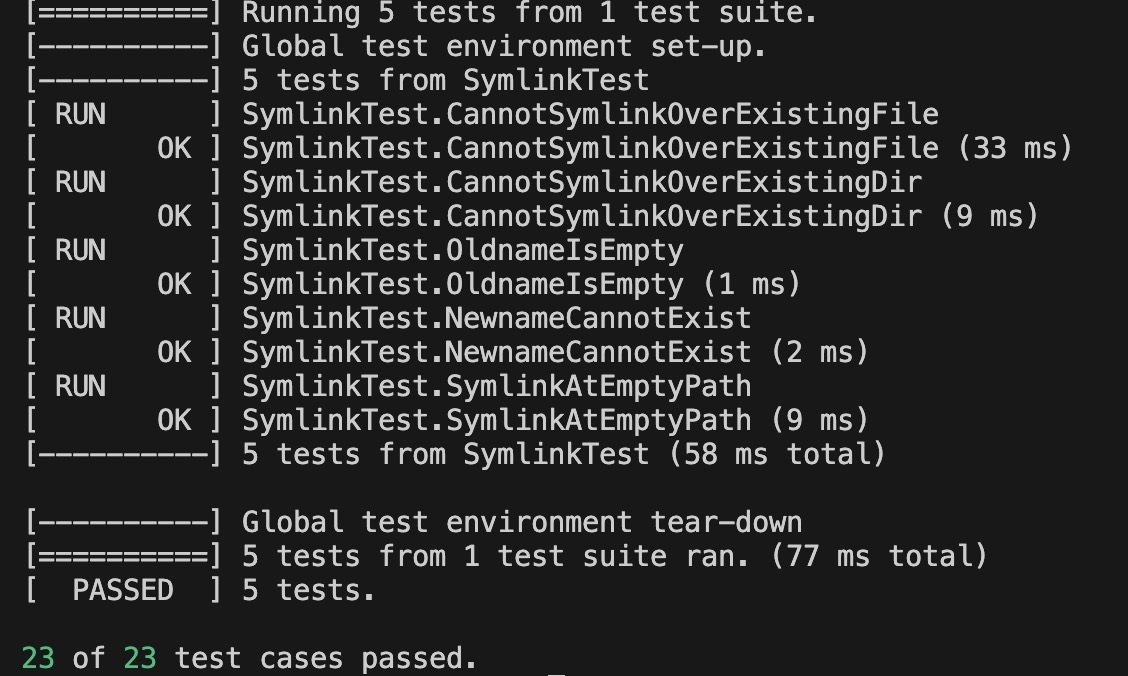
\includegraphics[width=1.0\textwidth]{chap5_gen_test.jpg}
    \caption{集成测试结果}
    \label{fig:gen_test}
\end{figure}
% vim:ts=4:sw=4
